\documentclass[final]{beamer}

\usepackage[orientation=portrait,size=a0,scale=1.6]{beamerposter}
\usepackage[utf8]{inputenc}
\usepackage[T1]{fontenc}
\usepackage[ngerman]{babel}
\usepackage{xcolor}
\usepackage{tikz}
\usepackage{lmodern}
\usepackage{booktabs}
\usepackage{tabularx}
\usepackage{graphicx}
\usepackage{pifont}

\definecolor{primary}{HTML}{4F6EF7}
\definecolor{dark}{HTML}{1A1D2E}
\definecolor{muted}{HTML}{6B7280}
\definecolor{soft}{HTML}{F0F2FF}
\definecolor{accent}{HTML}{818CF8}
\definecolor{warm}{HTML}{B45309}

\usetheme{default}
\setbeamercolor{background canvas}{bg=white}
\setbeamercolor{block title}{fg=white,bg=primary}
\setbeamercolor{block body}{fg=dark,bg=soft}
\setbeamercolor{block title alerted}{fg=white,bg=dark}
\setbeamercolor{block body alerted}{fg=dark,bg=soft}
\setbeamerfont{block title}{size=\LARGE,series=\bfseries}
\setbeamerfont{block body}{size=\large}
\setbeamertemplate{navigation symbols}{}

\newlength{\sepwidth}\setlength{\sepwidth}{0.04\textwidth}
\newcommand{\lw}{0.46\textwidth}

\begin{document}
\begin{frame}[t]{}

% ── HEADER ───────────────────────────────────────────────────────────────────
\begin{tikzpicture}[remember picture,overlay]
  \fill[primary] (current page.north west)
    rectangle ([yshift=-24cm]current page.north east);
\end{tikzpicture}

\vspace{1.0cm}
{\color{white}\fontsize{52}{62}\selectfont\bfseries
  Kognitive Beanspruchung bei\\[0.3cm]
  Datenvisualisierungen analysieren}\\[0.6cm]
{\color{white}\fontsize{24}{30}\selectfont
  Jonas Kimmer · Wirtschaftsinformatik M.Sc. · Hochschule RheinMain · 2026}\\[0.3cm]
{\color{soft}\fontsize{20}{26}\selectfont
  Betreuung: M.Sc. Yasmina Tajja \quad|\quad j.kimmer@student.hs-rm.de}
\vspace{2.0cm}

% ── 2 SPALTEN ────────────────────────────────────────────────────────────────
\begin{columns}[T]

%% LINKE SPALTE
\begin{column}{\lw}

  \begin{alertblock}{Forschungsfrage}
    \vspace{0.3em}
    \LARGE\bfseries
    Hängt kognitive Beanspruchung vom Thema ab,\\
    und misst Bearbeitungszeit wirklich mentale Last?
    \vspace{0.3em}
  \end{alertblock}

  \vspace{0.8em}

  \begin{block}{Beitrag dieser Arbeit}
    \vspace{0.4em}
    {\large
    \textcolor{primary}{\bfseries Tool\enskip}—\enskip
      Streamlit · Python · Einlesen · Segmentieren · Export\\[0.5em]
    \textcolor{primary}{\bfseries Daten\enskip}—\enskip
      NASA-TLX · Shimmer3 (GSR/PPG) · Tobii Eye-Tracker\\[0.5em]
    \textcolor{primary}{\bfseries Ergebnis\enskip}—\enskip
      18 Personen · 15 Aufgaben · 3 Domänen · Statistik
    }
    \vspace{0.3em}
  \end{block}

  \vspace{0.8em}

  \begin{block}{Länger brauchen → frustrierter, nicht belasteter}
    \vspace{0.3em}
    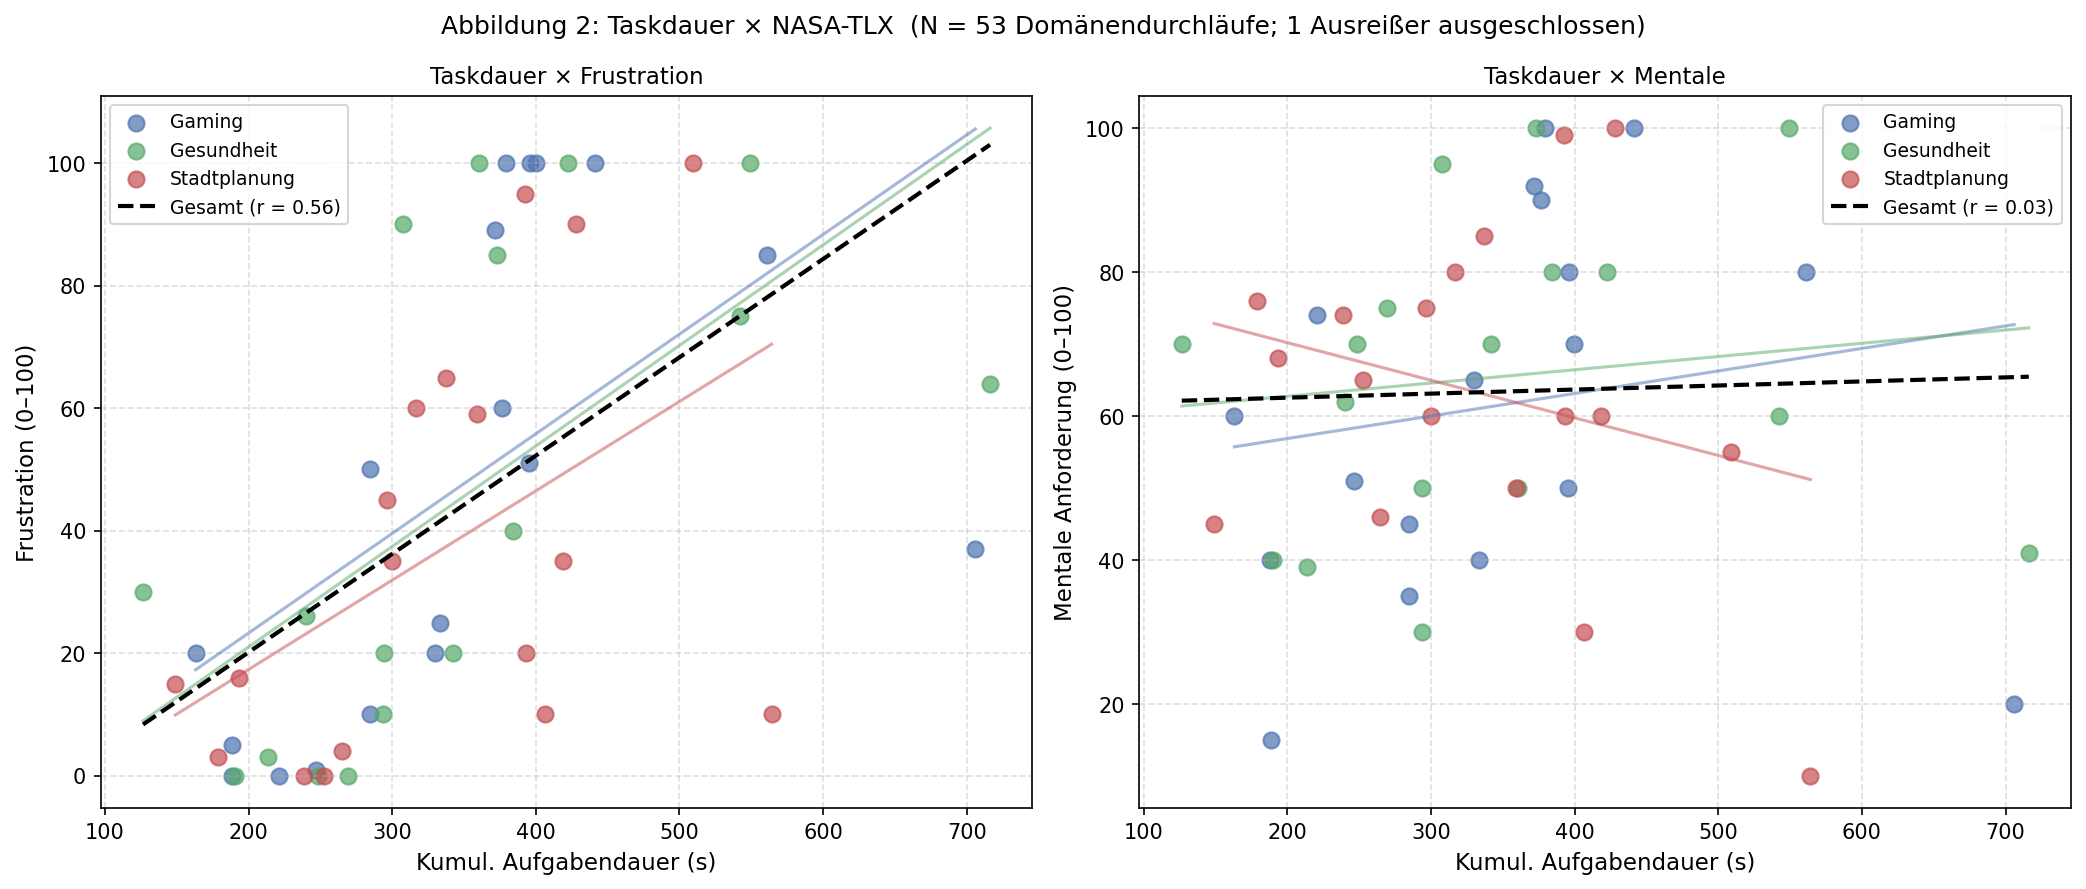
\includegraphics[width=0.98\linewidth]{figures/paper1_abb2_scatter_duration_tlx.png}
    \vspace{0.2em}
    {\large\color{muted}
    Pearson r\,=\,,56 (Frustration) · r\,=\,,03 (mentale Last)}
  \end{block}

\end{column}

\hspace{\sepwidth}

%% RECHTE SPALTE
\begin{column}{\lw}

  \begin{block}{3 Befunde}
    \vspace{0.4em}

    \begin{tikzpicture}
      \node[fill=primary,rounded corners=8pt,inner sep=12pt,
            text width=0.92\linewidth]{
        \color{white!70!primary}\large\bfseries
        \ding{172} Mentale Last (0--100 Pkt.)\\[0.4em]
        \color{white}\large
        · Gaming: \textbf{62} · Gesundheit: \textbf{63} · Stadtplanung: \textbf{63 Pkt.}\\[0.4em]
        \mdseries
        → Unterschied: nur \textbf{1,7 Punkte} — Fachwissen schützt nicht.
      };
    \end{tikzpicture}

    \vspace{0.6em}

    \begin{tikzpicture}
      \node[fill=dark,rounded corners=8pt,inner sep=12pt,
            text width=0.92\linewidth]{
        \color{white!60!dark}\large\bfseries
        \ding{173} Frustration (0--100 Pkt.)\\[0.4em]
        \color{white}\large
        · Gaming: \textbf{47} · Gesundheit: \textbf{44} · Stadtplanung: \textbf{37 Pkt.}\\[0.4em]
        \mdseries
        → \textbf{10 Punkte} Unterschied (6× mehr als bei mentaler Last)\\
        Vertrautheit schützt nicht vor Frustration.
      };
    \end{tikzpicture}

    \vspace{0.6em}

    \begin{tikzpicture}
      \node[fill=warm,rounded corners=8pt,inner sep=12pt,
            text width=0.92\linewidth]{
        \color{white!70!warm}\large\bfseries
        \ding{174} Anstrengung \& gefühlte Leistung\\[0.4em]
        \color{white}\large
        · Anstrengung: Gaming\,\textbf{51} · Gesundheit\,\textbf{45} · Stadt\,\textbf{46}\\[0.2em]
        · Leistung: Gaming\,\textbf{41} · Gesundheit\,\textbf{42} · Stadt\,\textbf{50}\\[0.4em]
        \small\color{white!60!warm}Leistung: höher = schlechter empfunden\\[0.3em]
        \large\mdseries\color{white}
        → Gaming: meiste Anstrengung · Stadt: schlechteste Leistung.
      };
    \end{tikzpicture}

  \end{block}

  \vspace{0.8em}

  \begin{alertblock}{Was das bedeutet}
    \vspace{0.3em}
    \LARGE\bfseries
    Für gutes Visualisierungsdesign zählt\\
    die Gestaltung — nicht das Thema.\\[0.5em]
    \large\mdseries
    · Kognitive Last bleibt gleich, egal ob vertrautes Fachgebiet\\[0.3em]
    · Vertrautheit schützt nicht vor Frustration\\[0.3em]
    · Bearbeitungszeit misst Frustration, nicht Denkaufwand\\[0.3em]
    · Vertrautes Thema = mehr Aufwand; unbekanntes = schlechtere Leistung
    \vspace{0.3em}
  \end{alertblock}

\end{column}
\end{columns}

\end{frame}
\end{document}
